\begin{figure*}[t!]
\centering
\begin{subfigure}{.18\textwidth}
  \centering
  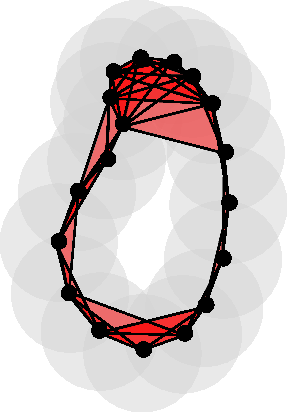
\includegraphics[width=.9\linewidth]{figure1_a.pdf}
\end{subfigure}
\hfill
\begin{subfigure}{.18\textwidth}
  \centering
  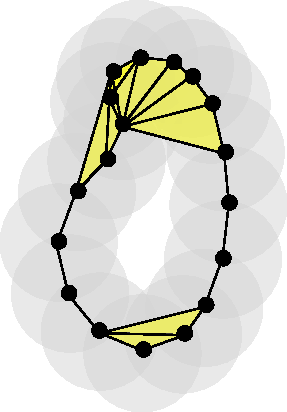
\includegraphics[width=.9\linewidth]{figure1_b.pdf}
\end{subfigure}
\hfill
\begin{subfigure}{.18\textwidth}
  \centering
  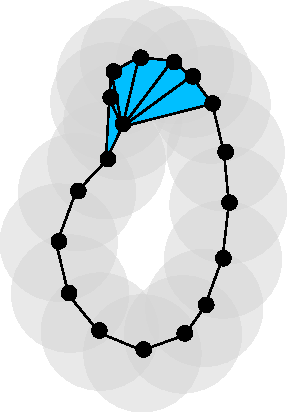
\includegraphics[width=.9\linewidth]{figure1_c.pdf}
\end{subfigure}
\hfill
\begin{subfigure}{.18\textwidth}
  \centering
  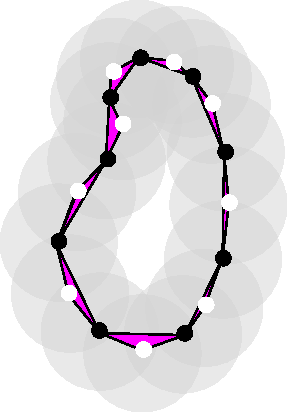
\includegraphics[width=.9\linewidth]{figure1_d.pdf}
\end{subfigure}
\hfill
\begin{subfigure}{.18\textwidth}
  \centering
  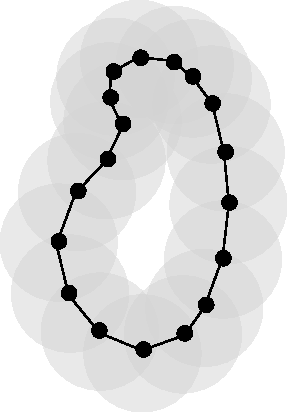
\includegraphics[width=.9\linewidth]{figure1_e.pdf}
\end{subfigure}
\caption{Four of five geometric complexes appearing in the collapsing sequence of the \v{C}ech-Delaunay Collapsing Theorem \cite{bauer2017morse}. From \textit{left} to \textit{right}: A high dimensional \v{C}ech complex projected onto the plane, the \v{C}ech-Delaunay complex, the Delaunay complex, the Witness complex, which is an outlier in the row due to the changing shape by different Witness sets (white bullets) and the Wrap complex.}
\label{fig:complexes}
\end{figure*}